\documentclass[a4paper,12pt]{article}
\usepackage[utf8]{inputenc}
\usepackage[T1]{fontenc}
\usepackage[spanish]{babel}
\usepackage{csquotes}
\usepackage{anysize}
\usepackage{graphicx}
\usepackage{hyperref}
%\usepackage{amsfonts}
%\usepackage{tikz}
%\usepackage{amsmath}
\marginsize{25mm}{25mm}{25mm}{25mm}

\title{Estadística inferencial}
\author{Daniel Maldonado}
\date{}

\begin{document}
{\scshape\bfseries \maketitle}

La estadística inferencial permite generalizar los resultados de muestras hacia poblaciones con niveles razonables de confianza.

Una hipótesis experimental podría ser que la media $\bar{X}$ del grupo al cual se aplicó una intervención es distinta de la media $\mu$ de la población de la cual se obtuvo la muestra. Es decir,
\begin{eqnarray*}
    \bar{X} &<& \mu\\
            &\mbox{o}&\\
    \bar{X} &>& \mu,
\end{eqnarray*}
o de forma más general:
\[
    \bar{X} \neq \mu
.\]

Suponemos que la muestra tenía originalmente la misma media que la población, y que la aplicación de nuestra intervención desplazó su media en una cierta dirección. En cierto modo, suponemos que nuestra intervención tiene el efecto de crear una segunda población con una media distinta de la población original.

Si la muestra fuese perfectamente representativa de la población original, entonces se podría concluir que si la media muestral $\bar{X}$ después del tratamiento es distinta de la media de la población $\mu$, entonces el tratamiento es eficaz. Sin embargo, la realidad no suele ser tan bella.

Una amenaza seria a la validez de la relación encontrada entre la aplicación del tratamiento experimental y el cambio en la media de la muestra es la posibilidad de un error de muestreo, es decir, que por azar la media de la muestra no fuese representativa de la población desde el comienzo. Esto tiene base en el {\slshape teorema central del límite} o {\slshape teorema del límite central}.

De acuerdo con el teorema podemos obtener muestras de una población y calcular la media de cada una de esas muestras. Si la cantidad de medias es lo bastante grande, entonces la distribución de esas medias tenderá a ser normal (una campana de Gauss) y la media formada por estas medias muestrales será muy cercana a la media $\mu$ de la población. Sin embargo, aunque las medias de las muestras tenderán a rondar el valor de la media poblacional, habrá una minoría que se encuentre muy lejos, ya sea por encima o por debajo. Así, existe una probabilidad nada despreciable de que la media de la muestra obtenida de la población esté muy por encima o muy por debajo del valor poblacional (Figura 1).

\begin{figure}[!ht]
  \begin{center}
    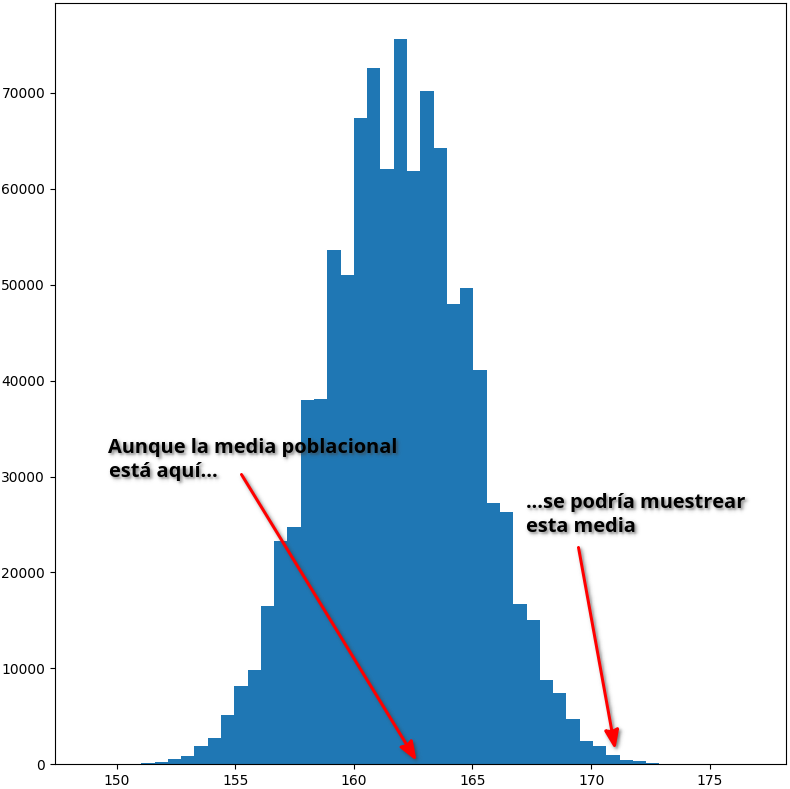
\includegraphics[scale=0.5]{curvaNormal.png}
    \caption{La media de la muestra puede estar en cualquier punto de la distribución.}
  \end{center}
\end{figure}

Si este fuera el caso, entonces la diferencia que encontramos entre la media $\bar{X}$ de la muestra tras el tratamiento y la media de la población $\mu$ sería solo debida al azar.

El papel de la estadística inferencial es garantizar que no cometamos el error de atribuir a la variable independiente (el tratamiento) las diferencias debidas a un error de muestreo.




\end{document}
